
\chapter{Implementacja systemu rekomendacyjnego}

WPROWADZENIE

\section{Fazy budowania systemu rekomendacyjnego}

Podczas implementacji systemu rekomendacyjnego wykorzystano typowy przepływ (przedstawiony na rysunku \ref{fig:rs_pipeline}) używany do tworzenia tego typu serwisów, który składa się z następujące pięć faz \cite{rs_in_real}:
\begin{itemize}
    \item wstępne przetwarzanie - na ten etap składają się czynności związane z transformacją danych do macierzy użytkownik-produkt oraz normalizacja w celu spłaszczenia wartości odstających (użytkownicy, którzy są nad wyraz pozytywni oraz negatywni w stosunku do dawania ocen),
    \item trenowanie - proces budowania modelu,
    \item optymalizacja hiper parametrów - wielokrotne trenowanie w celu dostrojenia parametrów w taki sposób, aby uzyskać jak najlepsze wyniki,
    \item przetwarzanie końcowe - sortowanie danych w celu uzyskania N najlepszych rekomendacji dla użytkownika, filtrowanie oraz wykluczenie wcześniej zakupionych lub negatywnie ocenionych przedmiotów,
    \item ewaluacja - testowanie stworzonego modelu poprzez ukrywanie/maskowanie ocen, a następnie użycie miar do ewaluacji (szczegółowo opisane w podrozdziale \ref{metryki}).
\end{itemize}{}

\begin{figure}
    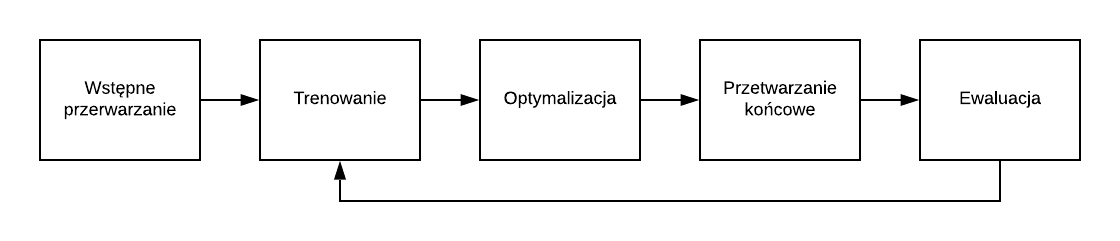
\includegraphics[scale=0.85]{rs_pipeline.png}
    \caption{Fazy przepływu podczas tworzenia systemu rekomendacyjnego.}
    \label{fig:rs_pipeline}
\end{figure}

\section{Dane testowe}